\documentclass{beamer}
\usecolortheme{default}
\usetheme{Madrid}

\usepackage{graphicx}
\usepackage{subfigure}

% Preamble
\title{LaTeX Cheat Sheet}
\author{Tratech GASS KNUST}
\date{\today}


% Body
\begin{document}
	% Variables
	\newcommand{\imgHeight}{100pt}
	\newcommand{\imgWidth}{100pt}
	
	\begin{frame}
		\titlepage
	\end{frame}
	
	\begin{frame}
		\tableofcontents
	\end{frame}
	
	\section{Document structure Commands}
	\begin{frame}{ Document Structure Commands}
		\begin{itemize}
			\item \texttt{\textcolor{blue}{\textbackslash documentclass\{...\}}} - To specify the overall layout of a document.
			\item \texttt{\textcolor{blue}{\textbackslash title\{...\}}} - Sets the main title of the document.
			\item \texttt{\textcolor{blue}{\textbackslash author\{...\}}} - Sets the author of the document.
			\item \texttt{\textcolor{blue}{\textbackslash date\{\textbackslash today\}}} - Sets the date to the current date.
			\item \texttt{\textcolor{blue}{\textbackslash begin\{document\}}} - Initiates the document structure.
			\item \texttt{\textcolor{blue}{\textbackslash maketitle}} - To display the preamble i.e. title, author , date ...
			\item \texttt{\textcolor{blue}{\textbackslash tableofcontents}} - For table of contents
		\end{itemize}
		
	\end{frame}
	
	\section{Content Commands and Usage}
	\begin{frame}{ Content Commands and Usag}
		\begin{itemize}
			\item \texttt{\textcolor{blue}{\%} - Indicate a comment}
			\item \texttt{\textcolor{blue}{\textbackslash par} -  It is used to create line breaks, similar to pressing "Enter" in a word processor}
			\item \texttt{\textcolor{blue}{\textbackslash noindent} - To suppress the indentation}
			\item \texttt{\textcolor{blue}{\textbackslash hspace} - To give a space horizontally}
			\item \texttt{\textcolor{blue}{\textbackslash vspace} - To give a space vertically}
			\item \texttt{\textcolor{blue}{\textbackslash centering}} - To center block of text, images or diagrams etc.
		\end{itemize}
	\end{frame}

	\section{Formatting Commands and Usage}
	\begin{frame}{ Formatting Commands and Usage}
		\begin{itemize}
			\item \texttt{\textcolor{blue}{\textbackslash textbf\{...\}} - Used to make the enclosed text bold}
			\item \texttt{\textcolor{blue}{\textbackslash textit\{...\}} - Used to make the enclosed text italic}
			\item \texttt{\textcolor{blue}{\textbackslash underline\{...\}} -  Used to underline the enclosed text.}
		\end{itemize}
	\end{frame}

	\section{Section Commands and Usage}
	\begin{frame}{Section Commands and Usage}
		\begin{itemize}
			\item \texttt{\textcolor{blue}{\textbackslash section\{...\}}} - To define a new section in the document
			\item \texttt{\textcolor{blue}{\textbackslash subsection\{...\}}} - To define a new section under the main section
			\item \texttt{\textcolor{blue}{\textbackslash subsubsection\{...\}}} - To define a new section under the subsection
			\item \texttt{\textcolor{blue}{\textbackslash section *\{...\}}} - To create an unnumbered section or heading
		\end{itemize}
		
	\end{frame}

	\section{List Commands and Usage}
	\begin{frame}{List Commands and Usage}
		\begin{itemize}
			\item \texttt{\textcolor{blue}{\textbackslash begin\{itemize\}}} - Starts a bulleted list environment.
			\item \texttt{\textcolor{blue}{\textbackslash begin\{enumerate\}}} - Initiates a numbered list environment.
			\item \texttt{\textcolor{blue}{\textbackslash begin\{equation\}}} - Begins a mathematical equation environment.
			\item \texttt{\textcolor{blue}{\textbackslash begin\{table\}}} - Initiates a table environment.
			\item \texttt{\textcolor{blue}{\textbackslash begin\{figure\}}} - Starts a figure or graphic environment.
		\end{itemize}
		
	\end{frame}


	\section{Math Commands and Usage}
	\begin{frame}{Math Commands and Usage}
		\begin{itemize}
			\item \texttt{\textcolor{blue}{\$ ... \$}} - For inserting mathematical expressions within a line a text \\ [10pt]
			\item \texttt{\textcolor{blue}{\textbackslash[ ... \textbackslash]}} - For inserting mathematical expressions to appear as a centered equation on its own line
			\item \texttt{\textcolor{blue}{\textbackslash dots}} - For 3 dots (...)
			\item \texttt{\textcolor{blue}{\textbackslash sqrt\{...\}}} - For inserting square root
		\end{itemize}
		
	\end{frame}

	\section{Images}
	\begin{frame}{Figures, Images Commands and Usage}
		\begin{itemize}
			\item \texttt{\textcolor{blue}{\textbackslash usepackage\{graphicx\}}} - Importing the graphic\textcolor{blue}{x} package
			\item \texttt{\textcolor{blue}{\textbackslash usepackage\{subfigure\}}} - Importing subfigures under a main figure
			
			\item \texttt{\textcolor{blue}{\textbackslash begin\{figure\}}} ... \texttt{\textcolor{blue}{\textbackslash end\{figure\}}} - To Insert images, diagrams or illustrations
			\item \texttt{\textcolor{blue}{\textbackslash centering}} - To center images, diagrams, illustrations or even block of text
			
			\item \texttt{\textcolor{blue}{\textbackslash includegraphics\{image.jpg\}}} - To include external files eg. images
			\item \texttt{\textcolor{blue}{\textbackslash caption\{Eg. This is an image\}}} - To indicate a caption
			
			
		\end{itemize}
	\end{frame}
	\begin{frame}{Formatting the image}
		\begin{itemize}
			\item \texttt{\textcolor{blue}{\textbackslash includegraphics[height=200pt, width=100pt]\{image.jpg\}}} - Including a figure and specifying the height and width
			
			\item \texttt{\textcolor{blue}{\textbackslash begin\{figure\}[!t]}} ... \texttt{\textcolor{blue}{\textbackslash end\{figure\}}} - Place the image at the top of the page
			
			\item \texttt{\textcolor{blue}{\textbackslash begin\{figure\}[!b]}} ... \texttt{\textcolor{blue}{\textbackslash end\{figure\}}} - Place the image at the bottom of the page
			
			\item \texttt{\textcolor{blue}{\textbackslash begin\{figure\}[!here]}} ... \texttt{\textcolor{blue}{\textbackslash end\{figure\}}} - Place the image at the exact place of the editor \textcolor{blue}{( h means here)}
			
			\item \texttt{\textcolor{blue}{\textbackslash subfigure\{\textbackslash includegraphics\{image.jpg\}\}}} - To add a subimage or a subfigure
			
			\item \texttt{\textcolor{blue}{\textbackslash subfigure[This is a subcaption]\{\textbackslash includegraphics\{image.jpg\}\}}} - To add a sub caption to a figure
			
		\end{itemize}
	\end{frame}

	\begin{frame}{Inserting image example}
		\begin{figure}[!t]
			\centering
				\subfigure[Mass Passport]{
\includegraphics[height=100pt, width=100pt]{images/fliers/passport.jpg}} \hspace{5pt}
				\subfigure[Event Calendar]{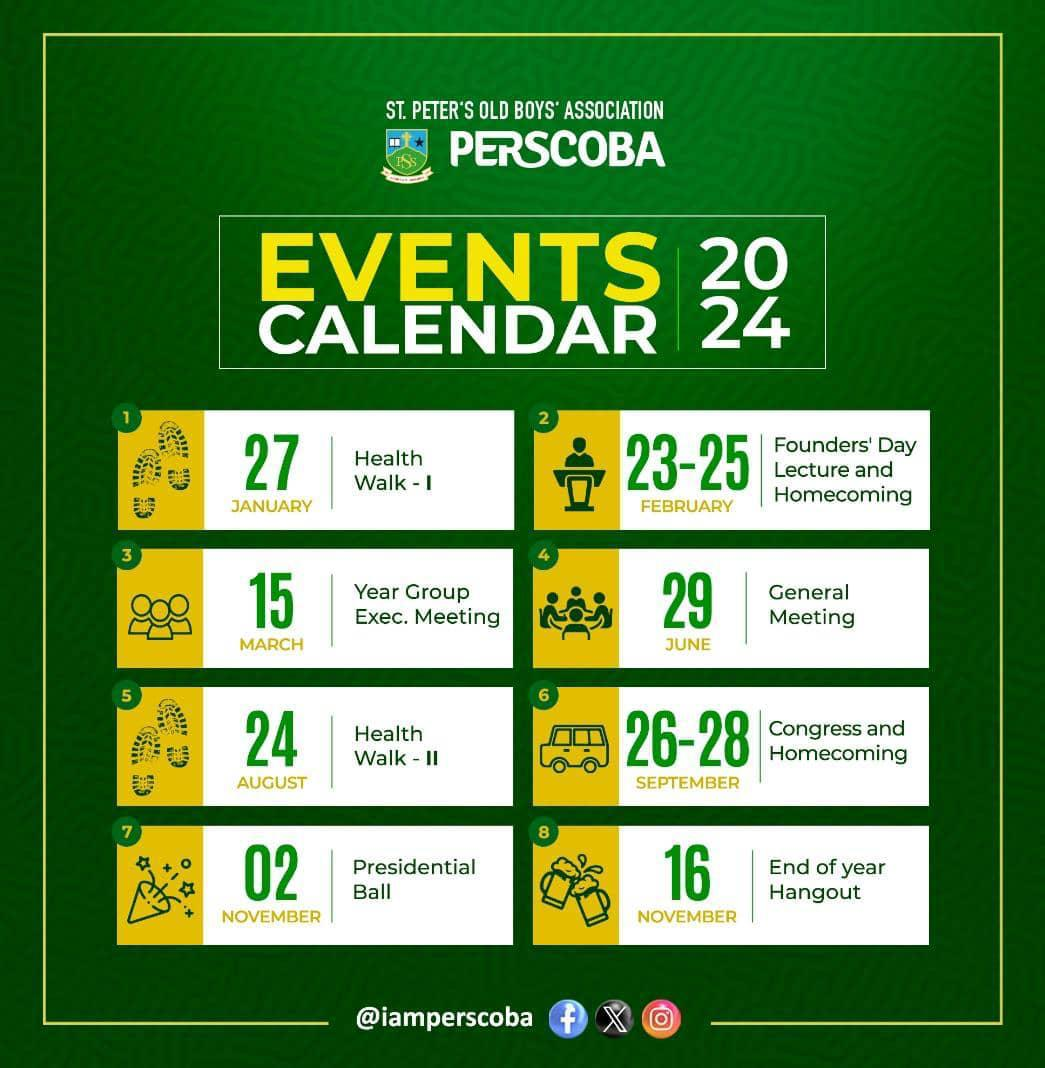
\includegraphics[height=100pt, width=100pt]{images/fliers/persco_event.jpg}}
			
			\caption{Fliers}
			\label{fig:figure1}
		\end{figure}
	\end{frame}
	\begin{frame}{LaTeX Code for inserting image}
		\begin{figure}
			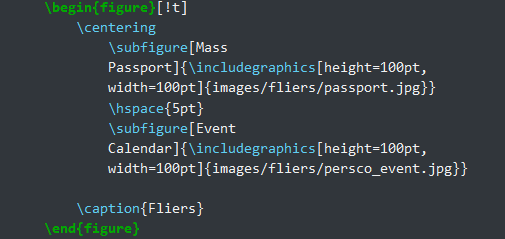
\includegraphics[width=0.9\textwidth, height=0.6\textheight]{images/code/fliers_code.png}
			
			\caption{Code for inserting image (\ref{fig:figure1}) }
		\end{figure}
	\end{frame}
	
	
	% Add more frames for additional commands...
	
\end{document}
